\chapter{实现效果}

机器人外形如下

\begin{figure}[h]
        \centering
                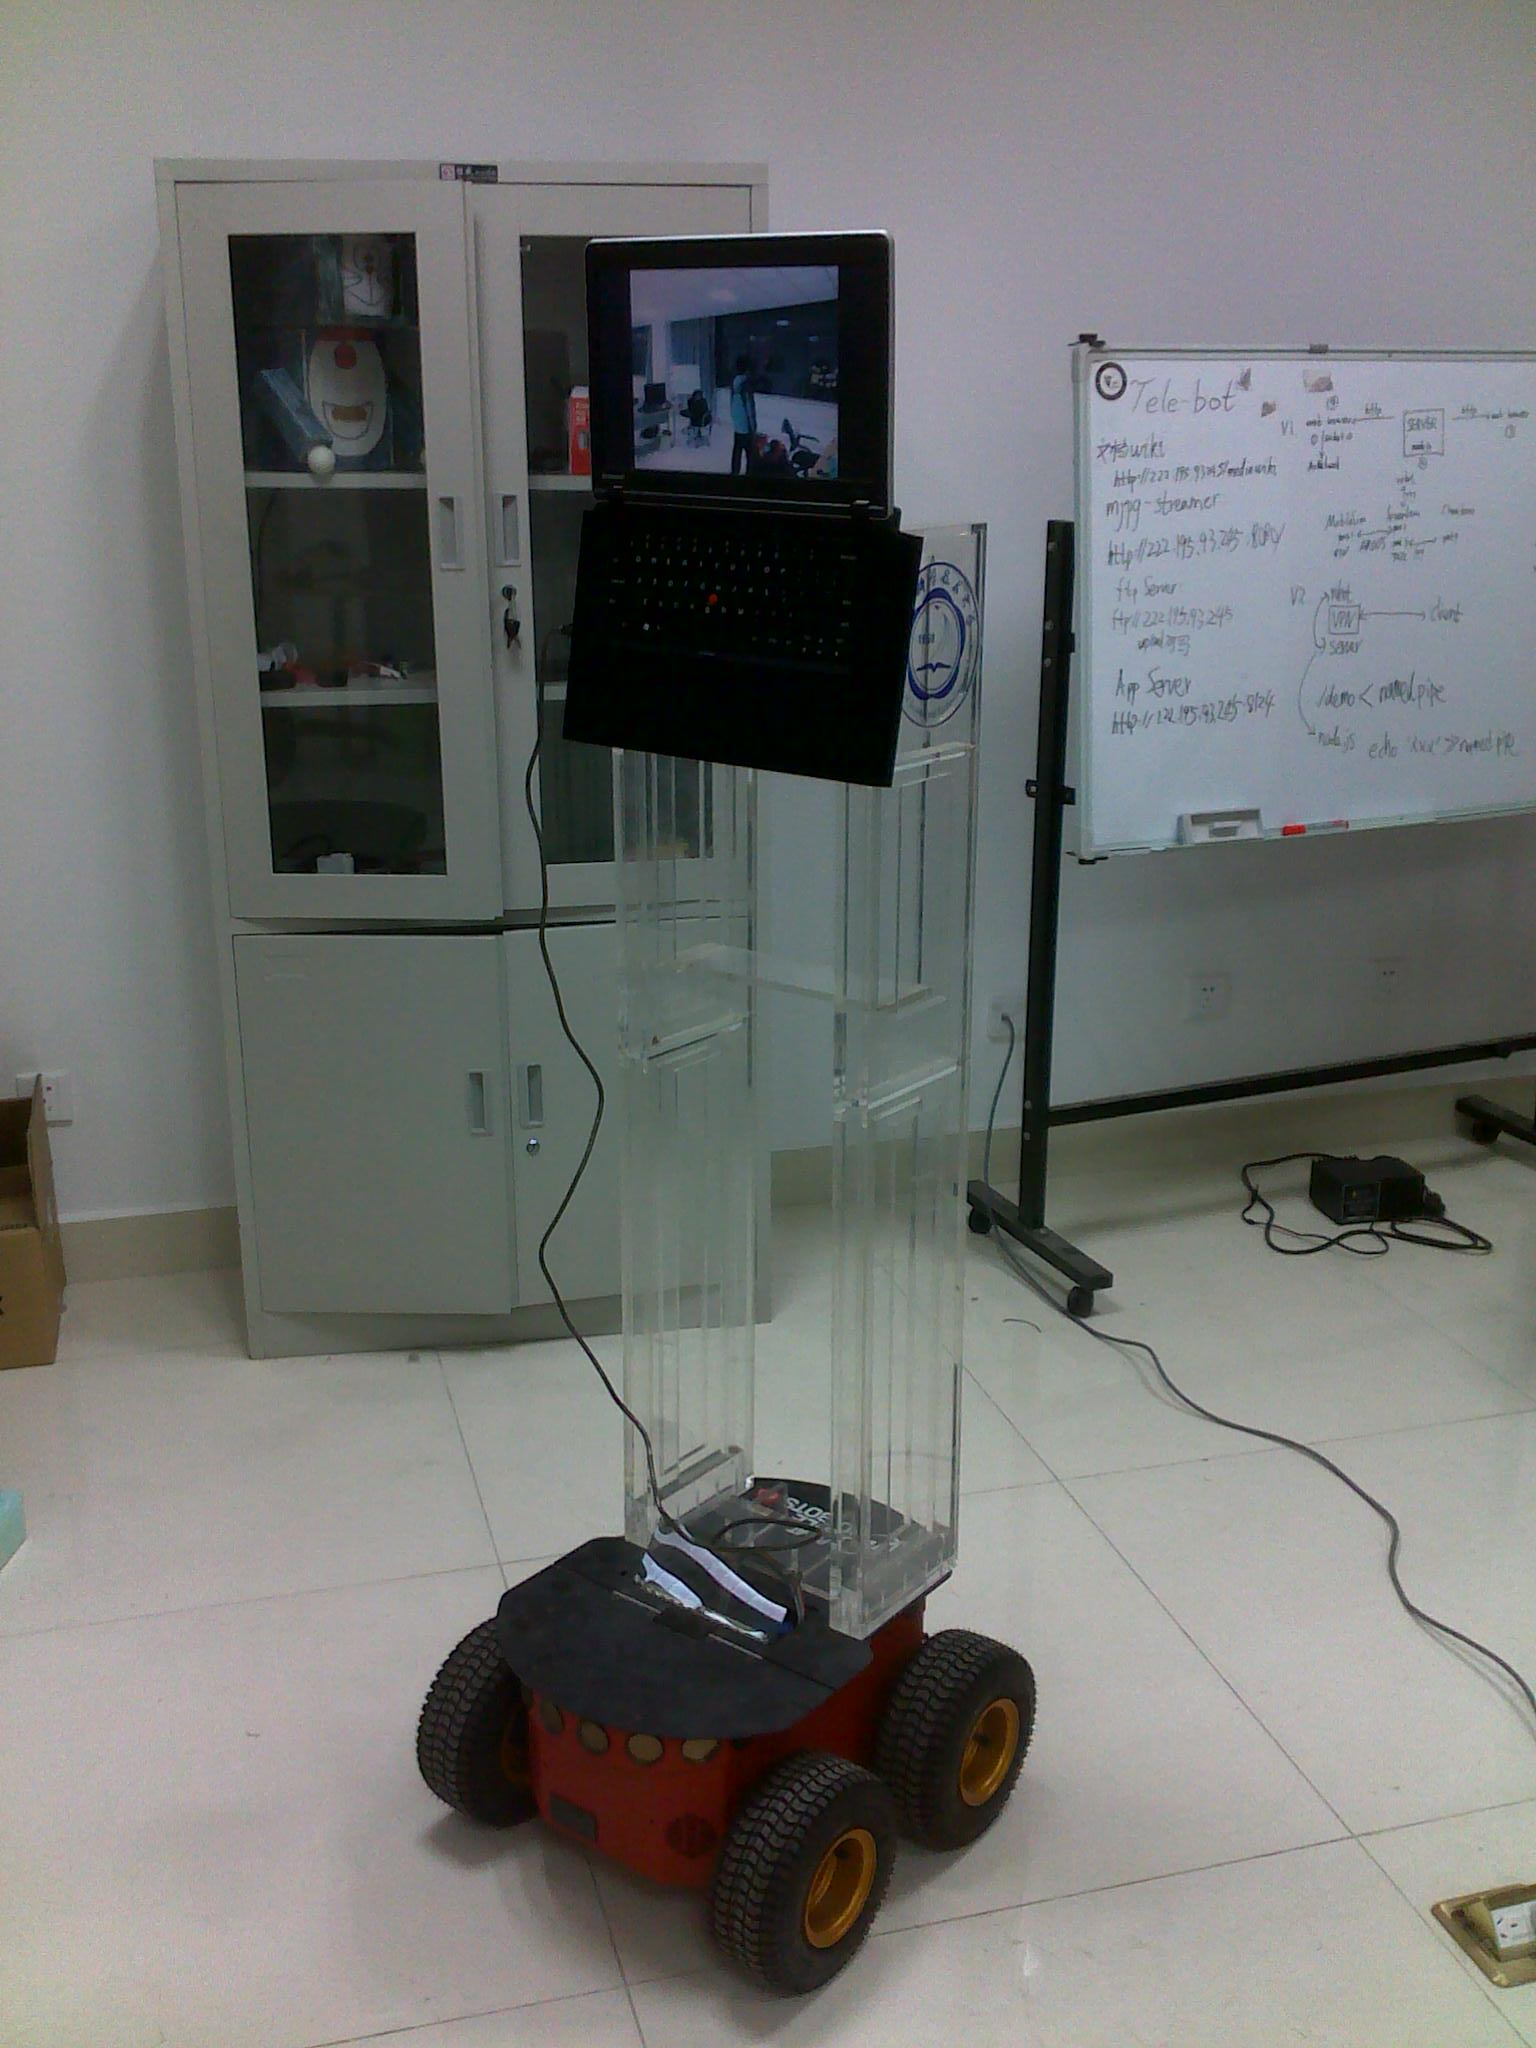
\includegraphics[width=.70\textwidth]{Figures/ch9.outlook.jpg}
        \caption{机器人外观}
        \label{fig:outlook}
\end{figure}

用户端主界面如下

\begin{figure}[h]
        \centering
                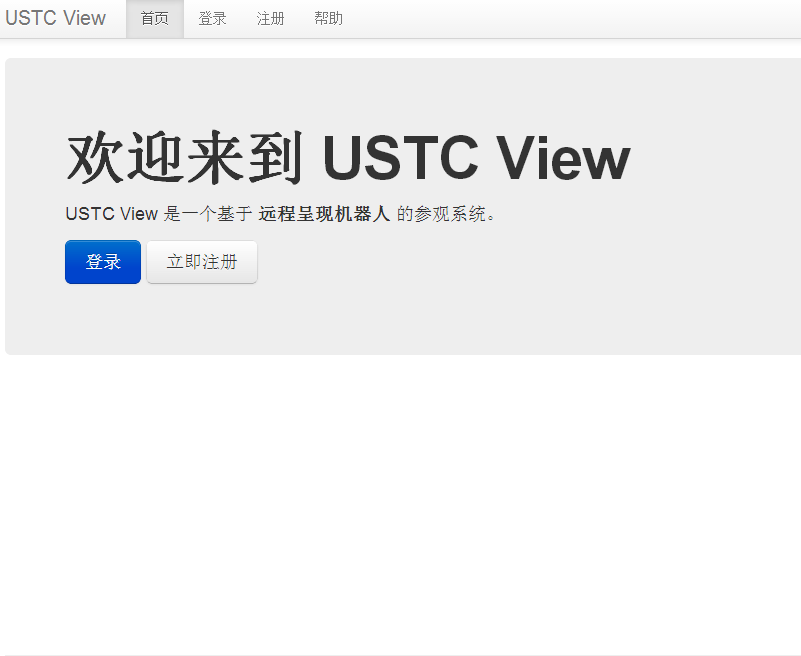
\includegraphics[width=.70\textwidth]{Figures/ch9.ui.png}
        \caption{用户界面}
        \label{fig:UI}
\end{figure}

这是登入服务页面的效果图,用户通过点击注册来获得有权限的账号。

点击帮助按钮会提供一段视频,展示该服务的使用具体使用方法。

用户登录之后,便进入到相应的有使用权限的页面,如下图:

\begin{figure}[h]
        \centering
                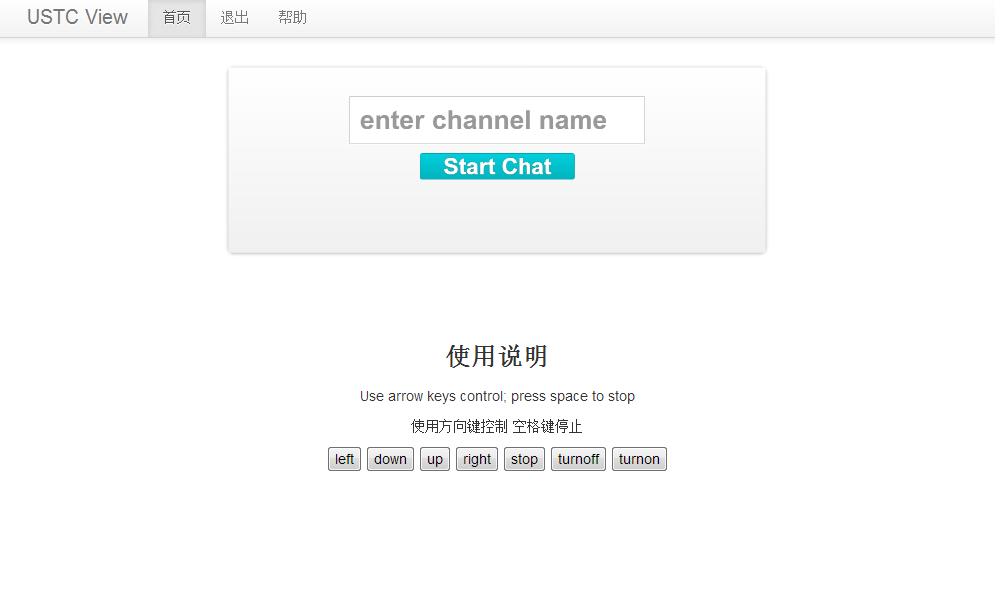
\includegraphics[width=.70\textwidth]{Figures/ch9.user.png}
        \caption{登录后界面}
        \label{fig:user}
\end{figure}

在channel name中输入机器人提供的相关channel信息,点击start即可开始音视频的通讯。
效果如下图,视频由机器人上的广角摄像头拍摄所得。

\begin{figure}[h]
        \centering
                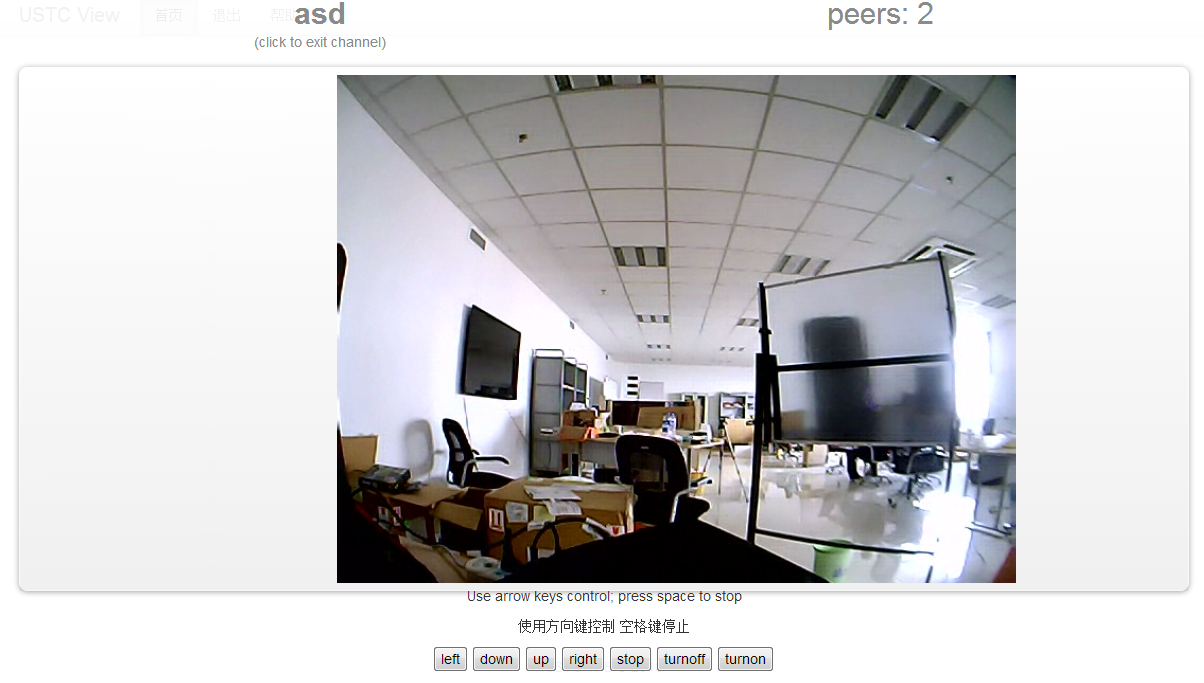
\includegraphics[width=.70\textwidth]{Figures/ch9.view.png}
        \caption{远程呈现}
        \label{fig:view}
\end{figure}

在该页面上,敲击方向键上下左右来控制移动,或者通过直接点击面板上的按钮来实现。
